\begin{figure}[H]
    \centering
    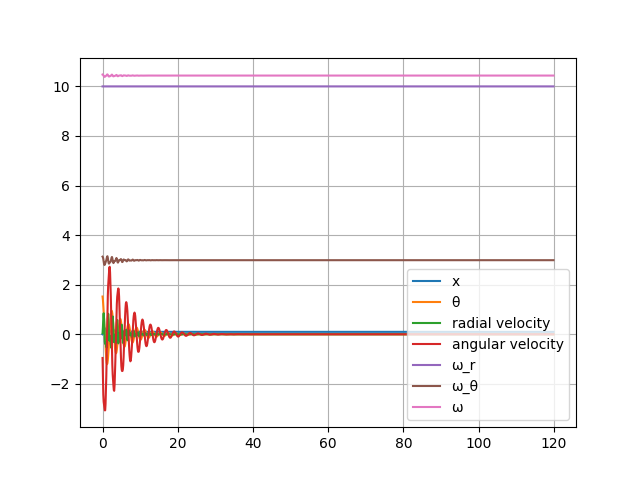
\includegraphics[width=15cm]{ExpPictures/m1.png}
    \caption{{Case 1 where m = 1 kg}}
    \label{}
\end{figure}
        
\begin{figure}[H]
    \centering
    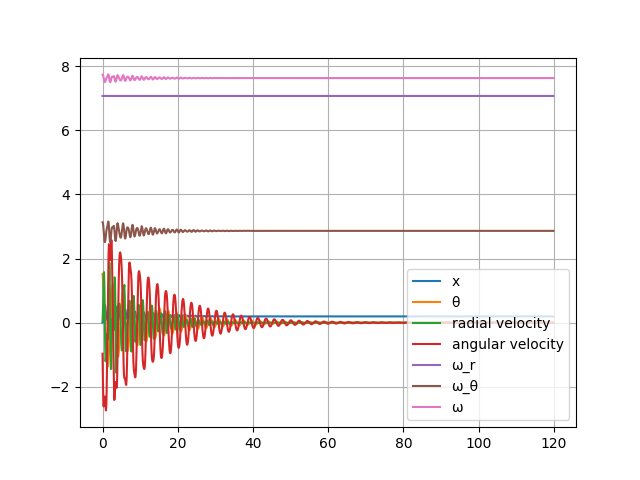
\includegraphics[width=15cm]{ExpPictures/m2.png}
    \caption{{Case 2 where m = 2 kg}}
    \label{}
\end{figure}
        
\begin{figure}[H]
    \centering
    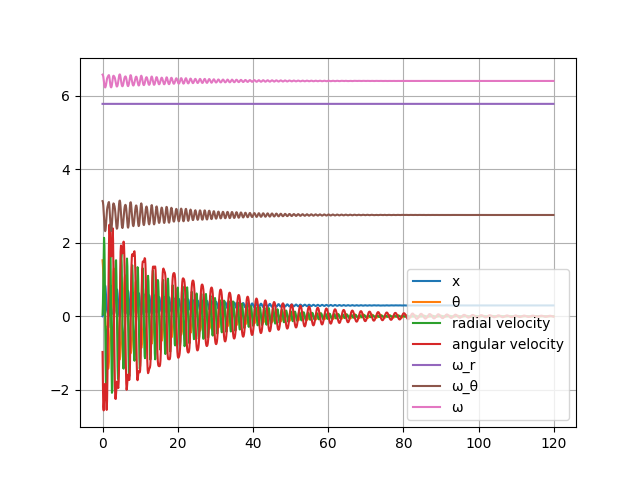
\includegraphics[width=15cm]{ExpPictures/m3.png}
    \caption{{Case 3 where m = 3 kg}}
    \label{}
\end{figure}
        
\begin{figure}[H]
    \centering
    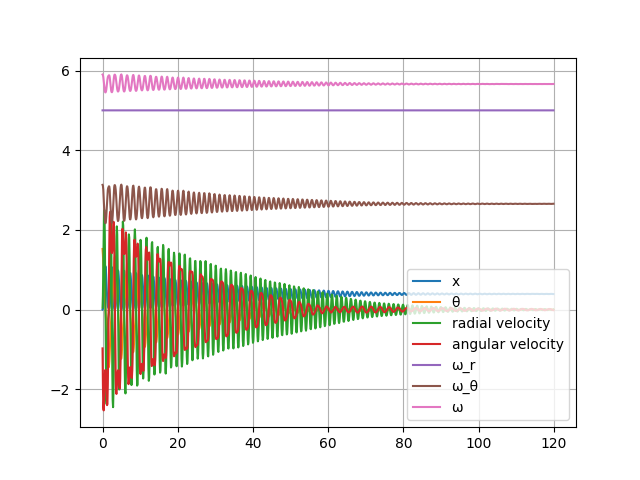
\includegraphics[width=15cm]{ExpPictures/m4.png}
    \caption{{Case 4 where m = 4 kg}}
    \label{}
\end{figure}
        
\begin{figure}[H]
    \centering
    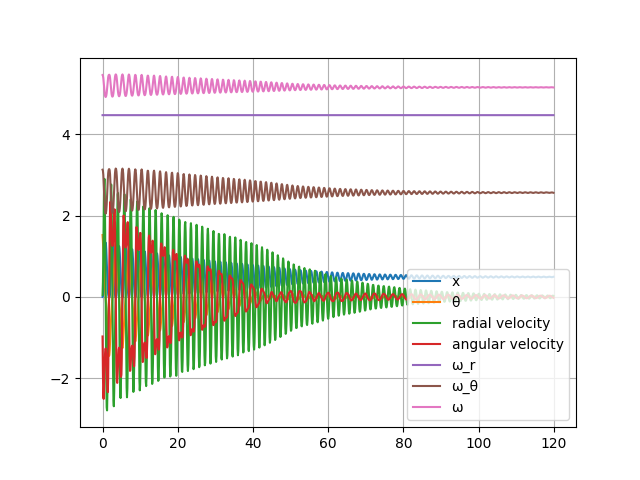
\includegraphics[width=15cm]{ExpPictures/m5.png}
    \caption{{Case 5 where m = 5 kg}}
    \label{}
\end{figure}
        
\begin{figure}[H]
    \centering
    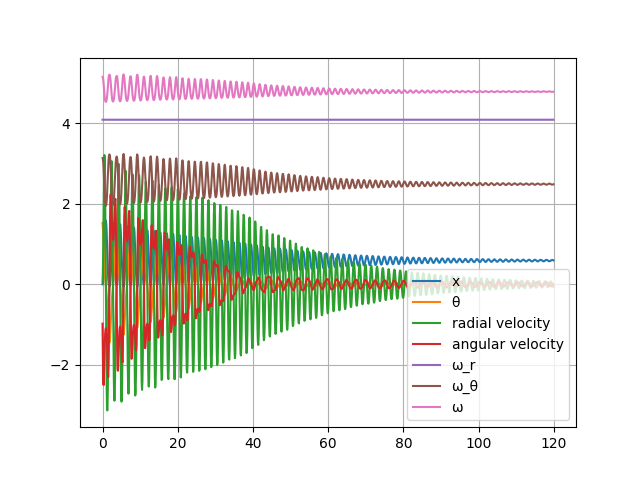
\includegraphics[width=15cm]{ExpPictures/m6.png}
    \caption{{Case 6 where m = 6 kg}}
    \label{}
\end{figure}
        
\begin{figure}[H]
    \centering
    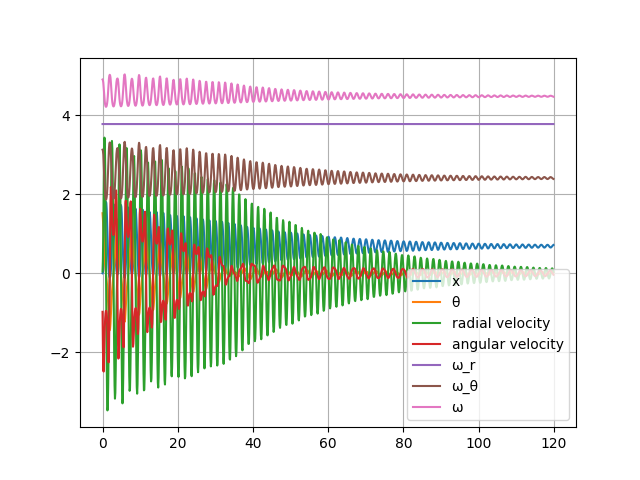
\includegraphics[width=15cm]{ExpPictures/m7.png}
    \caption{{Case 7 where m = 7 kg}}
    \label{}
\end{figure}
        
\begin{figure}[H]
    \centering
    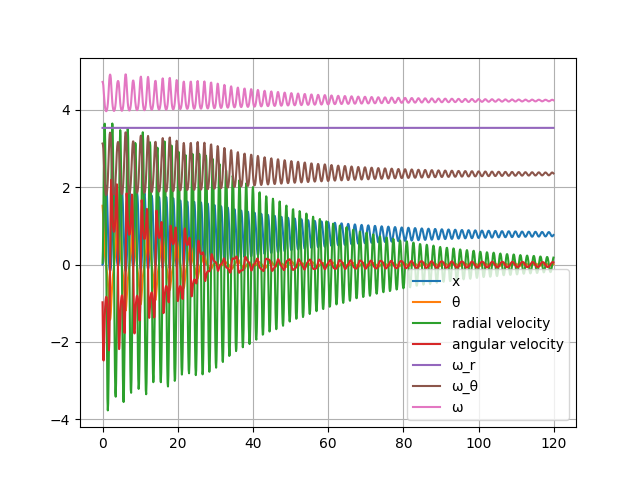
\includegraphics[width=15cm]{ExpPictures/m8.png}
    \caption{{Case 8 where m = 8 kg}}
    \label{}
\end{figure}
        
\begin{figure}[H]
    \centering
    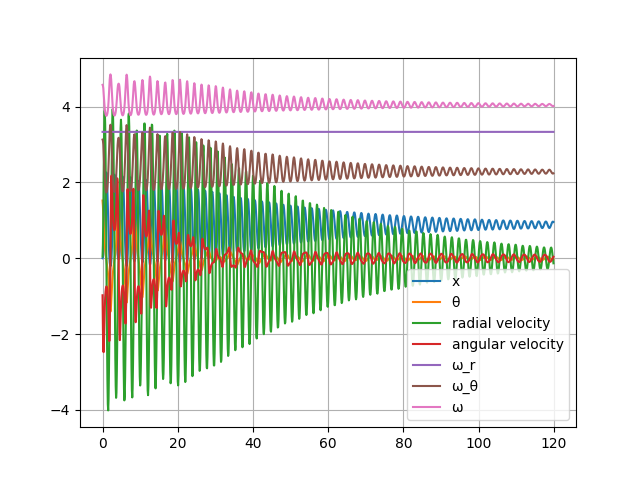
\includegraphics[width=15cm]{ExpPictures/m9.png}
    \caption{{Case 9 where m = 9 kg}}
    \label{}
\end{figure}
        
\begin{figure}[H]
    \centering
    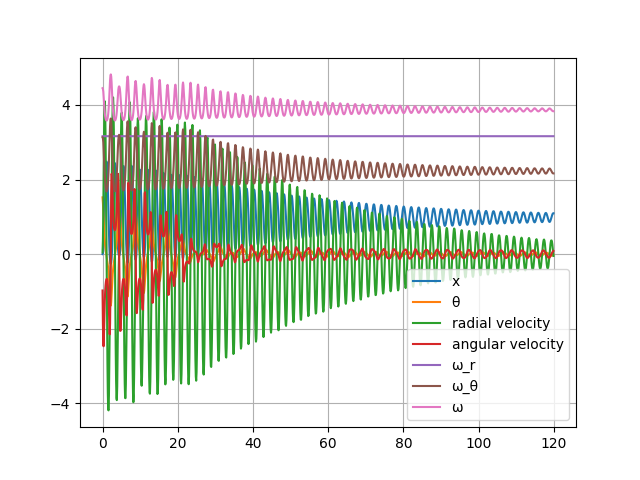
\includegraphics[width=15cm]{ExpPictures/m10.png}
    \caption{{Case 10 where m = 10 kg}}
    \label{}
\end{figure}
        





